\label{sec:cnninterrupt}
% The idea of interruption is introduced for dynamic multi-task scheduling. This section details the implementation of our \textbf{Virtual instruction Interruption}. \Cref{fig:interDPR} illustrates the idea of interruption to full utilize the hardware resources.

\begin{table*}[t]
	\footnotesize
	\centering
	\caption{Description for the basic instructions.}
% Table generated by Excel2LaTeX from sheet 'Sheet3'
\begin{tabular}{|p{2.7em}|p{3.4em}|p{16em}|p{4.2em}|p{4.6em}|p{4.2em}|p{4.2em}||p{7em}|p{7em}|}
	\hline
	\multicolumn{1}{|c|}{Category} & \multicolumn{1}{c|}{Type} & \multicolumn{1}{c|}{Description} & \multicolumn{1}{c|}{Address 1} & \multicolumn{1}{c|}{Address 2} & \multicolumn{1}{c|}{Address 3} & \multicolumn{1}{c||}{Workload} & \multicolumn{1}{c|}{Backups} & \multicolumn{1}{c|}{Recovery $^1$} \bigstrut\\
	\hline
	\multirow{2}[4]{*}{LOAD} & LOAD\_W & Load weights/bias from DDR to on chip weight buffer. & Off-chip Addr & Weights-buffer Addr & -     & Data  Length & -     & Weight / Inputdata \bigstrut\\
	\cline{2-9}\multicolumn{1}{|c|}{} & LOAD\_D & Load input data from DDR to on-chip data buffer. & Off-chip Addr & Data-buffer Addr & -     & Data  Length & -     & Weight / Inputdata \bigstrut\\
	\hline
	\multirow{2}[4]{*}{CALC} & CALC\_I & Calculate intermediate results (from partial input channels) for some output channels from partial  input channels. & Input  Data Addr & Intermediate Data Addr & Weight Addr & Calc Size & Previous final results / Intemediate data  & Weight / Inputdata /  intemediate data \bigstrut\\
	\cline{2-9}\multicolumn{1}{|c|}{} & CALC\_F & Calculate the results for some output channels from all input channels. The pooling, bias-adding and elementwise operations are operated in this instructions. & Input  Data Addr & Output  Data Addr & Weight Addr & Calc Size & Finial results & Weight / Inputdata \bigstrut\\
	\hline
	SAVE  & SAVE  & Save the results from on-chip data buffer to DDR. & Off-chip Addr & Data-buffer Addr & -     & Data  Length & -     & Weight / Inputdata \bigstrut\\
	\hline
	\end{tabular}%
	
	\label{tab:instr}%
  \end{table*}%


% \begin{figure*}[t]
% 	\centering
% 	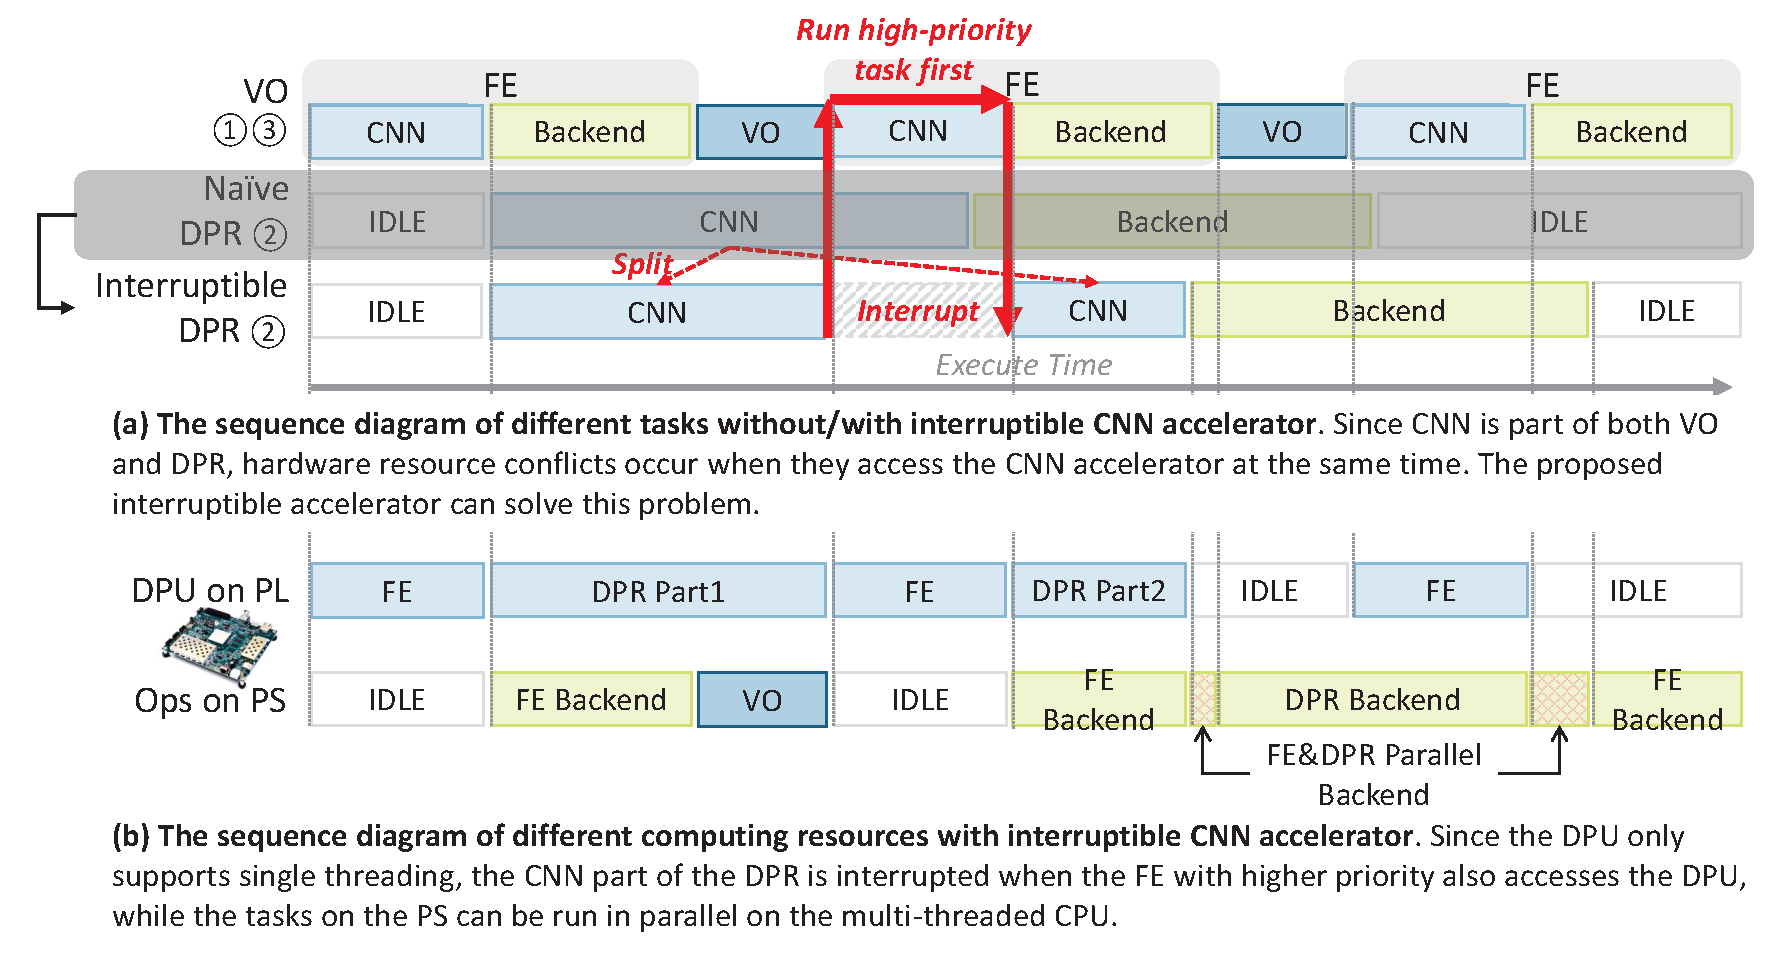
\includegraphics[width=0.9\linewidth]{fig/interDPR.eps}
% 	\caption{Interruption to solve the hardware resources conflicts.  When a high-priority task (FE) is started before the low-priority task (PR) is completed, the CNN accelerator backs up the status of PR to memory, and processes the FE task. When the high-priority task is completed, the low-priority task resumes and continues.
%     }
% 	\label{fig:interDPR}
% \end{figure*}

In this section, we introduce the concept of interrupt to CNN accelerator to support multi-task execution.

\subsection{Accelerator Interrupt}

In order to support multi-task scheduling, interrupt is introduced in CPU. 
In CPU, when a high-priority task requires an interrupt, the hardware or the interrupt handler software would back up the registers to main memory.
After the high-priority task is completed, the backed-up registers will be recovered to CPU hardware. 

If the CNN accelerator support interrupt, it can run two or more CNN modules at the same time. \Cref{fig:interDPR} illustrates the idea of interrupt to schedule two CNN tasks simultaneously. In the process of running a low-priority network (PR), the software may send an execution request for the high-priority task (FE). The interrupt enables the CNN accelerator to backup the running state of previous task low-priority PR network, and then execute the high-priority FE network. When the high-priority task (FE) is complete, the low-priority task (PR) is restored to the accelerator and continues to execute.

With the help of accelerator interrupt, the execution of the low-priority task (PR) is divided into pieces, and each piece is allocated to the time interval of running the high-priority networks (FE). 
Accelerator interrupt multiplexes the time division of the accelerator, reduces the idle time of the accelerator, and improves the utilization of hardware resources. 

\subsection{How To Interrupt: Virtual Instruction}
\label{sec:howinter}


However, the CPU-like interrupt would back up all the on-chip registers to DDR. In CPU, there are tens of registers, and the backed-up data is around 1 KB. In CNN accelerators, there are hundreds of KB ~ several MB on-chip cache \cite{qiu2016going, yu2018instruction}. If all the on-chip cache is backed-up and recovered, the cost of data transfer in the CNN accelerator is much higher than that of CPU.

We propose the \textbf{virtual-instruction-base} method to enable interrupt. The low-priority task maintains the executing status itself, rather than the hardware or the interrupt handler used in CPU. Only the cache which is still needed in future execution will be backed-up and restored.

The virtual instructions, which contain the backup and recovery instructions, are generated in the compilation phase, together with the normal instructions. 
For backup instructions, the corresponding input data and weights are still stored in DDR. 
There is no need to back up the input buffer and weight buffer, and only the intermediate data and the final output results are needed to be backed-up. 
For recovery instructions, the weights and input data for future calculation, as well as the backed-up intermediate data, are needed to be restored from DDR to the on-chip cache.

There is a field in the instruction set, that indicates whether the instruction a virtual instruction. If no interrupt occurs, virtual instructions will be skipped and discarded, which can ensure the efficiency of uninterrupted execution.

\subsection{ Where To Interrupt: After Save/CALC\_F }
\label{sec:whereinter}

There are three categories of instruction in the instruction-driven accelerator: LOAD, CALC, and SAVE. The instruction description and the backup/recovery data for interrupt position at each kind of instruction are listed in \Cref{fig:normal_instr} and \Cref{tab:instr}.

\begin{figure}[h]
	\centering
	
\includegraphics[width=0.9\linewidth]{fig/normal_instr.eps}
	\caption{The extended instruction set for virtual instruction }
	\label{fig:normal_instr}
\end{figure}

Each CALC instruction, including CALC\_I and CALC\_F processes the convolution from input feature of the hardware input parallelism ($Para_{in}$) to the output feature of the hardware output parallelism ($ Para_{out}$), as illustrated in \Cref{fig:calschedule}(a). The convolution of the last input channels is CALC\_F, and the convolutions for the former input channels are CALC\_I. The CALC\_F and the CALC\_I instructions to generate the output channels, as well as the LOAD instructions for corresponding input featuremaps and weights are considered as a \textbf{CalcBlob}.

The backup/recovery data transfer for interrupting each instruction is analyzed as follows:

\subsubsection{LOAD\_W / LOAD\_D }
When an interruption occurs at LOAD, the newly loaded data would immediately be flushed when running the high-level CNN, leading to bandwidth waste.

\subsubsection{CALC\_I} 
When an interrupt occurs at CALC\_I, the unsaved finial results ( generated by previous CALC\_F) should be saved to DDR. The intermediate data from current CALC\_I should also be sent to DDR for further use. At the Recovery stage, the intermediate data should be fetched from DDR. The data movement of intermediate results leads to additional bandwidth requirements.


\subsubsection{CALC\_F}
When an interrupt occurs at CALC\_F, there is no need to back up and recovery intermediate results. Although it is necessary to back up the unstored final results which are generated by previous CALC\_F, these results will be stored in DDR through the subsequent normal SAVE instruction.
If the accelerator can record the interrupt status, we can modify the address and workload when executing subsequent normal not-virtual save instruction.
In this way, we can avoid the repetitive transmission of results.
The state records and modifications to normal SAVE instruction will be introduced in the following subsections.

\begin{figure}[h]
	\centering
	
\includegraphics[width=0.99\linewidth]{fig/virtual_instr.eps}
	\caption{The basic structure of a instruction }
	\label{fig:virtual_instr}
\end{figure}



\begin{figure*}[t]
	\begin{minipage}[t]{0.49\linewidth}  
	\centering
	\subfigure[One Save for Single CALC/LOAD.] {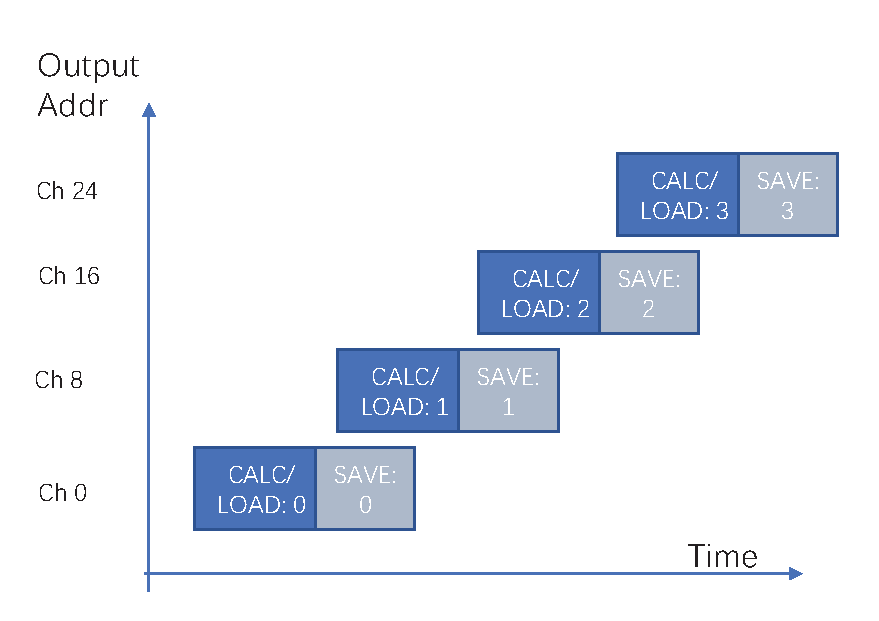
\includegraphics[width=0.9\linewidth]{fig/singlesave.eps}\label{fig:singlesave}}
	\end{minipage}
	\begin{minipage}[t]{0.49\linewidth}  
	\centering  
	\subfigure[One Save for Multiple CALC/LOAD.] {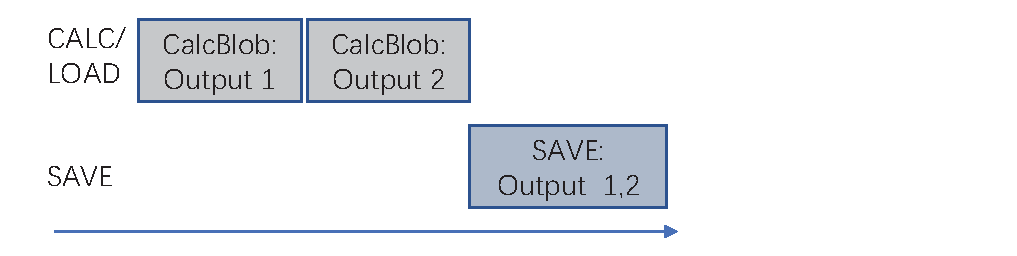
\includegraphics[width=0.9\linewidth]{fig/multisave.eps}\label{fig:multisave}} 

	\end{minipage}
	\begin{minipage}[t]{0.49\linewidth}  
	\centering  
	\subfigure[Interrupt for \Cref{fig:singlesave} ] {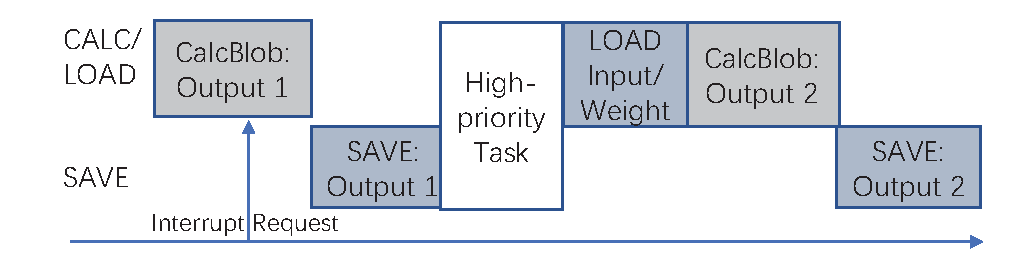
\includegraphics[width=0.9\linewidth]{fig/intersingle.eps}\label{fig:intersinglesave}} 
	\end{minipage}
	\begin{minipage}[t]{0.49\linewidth}  
	\centering  
	\subfigure[Interrupt for \Cref{fig:multisave}] {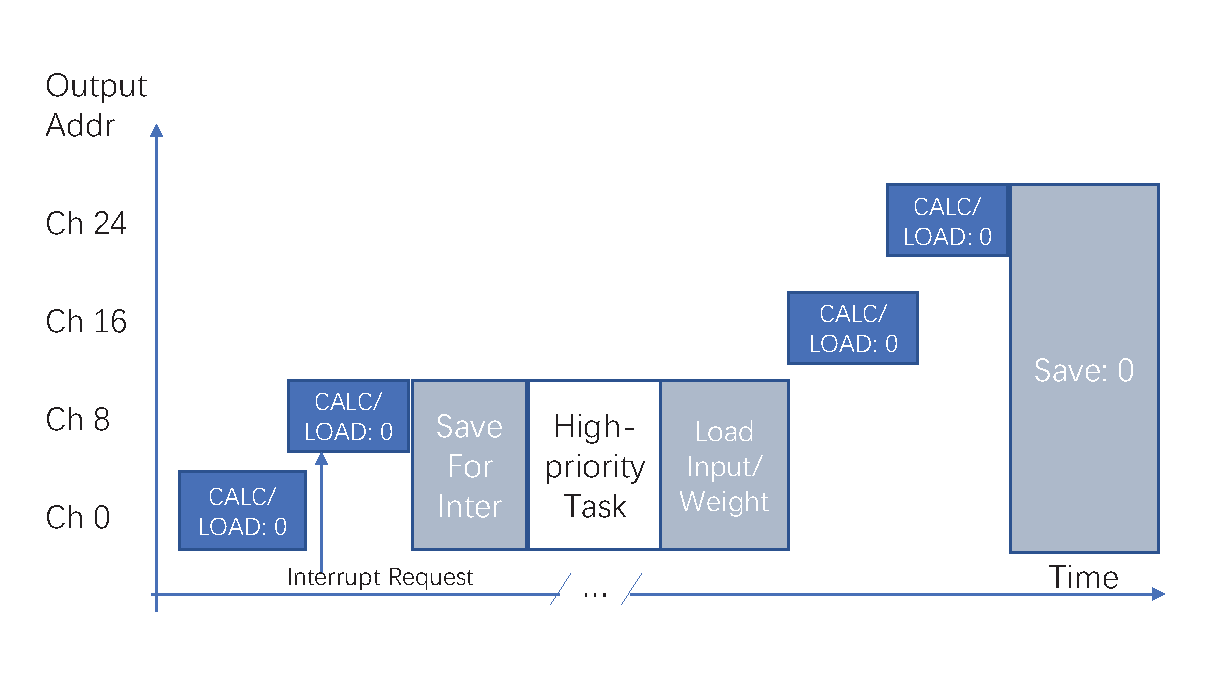
\includegraphics[width=0.9\linewidth]{fig/intermulti.eps}\label{fig:intermultisave}} 
	\end{minipage}
	\caption{ Scheduling Illustration
%   (d) find a single intra-robot loop closure which (c) and (d) cannot find, so that the result is better than (c) and (e).
  }
\label{fig:dslamresult}
\end{figure*}


\begin{figure}[t]
	\centering
	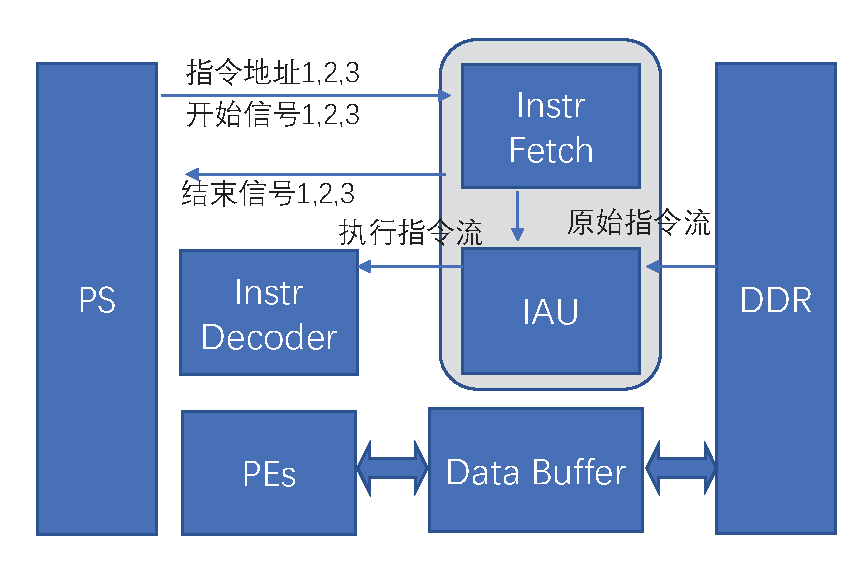
\includegraphics[width=0.99\linewidth]{fig/iau.eps}
	\caption{Hardware Architecture of IAU. The software on the CPU side (PS side) communicates IAU to access the CNN accelerator. IAU records the running state of each task, such as the address to fetch instructions, the SaveID of interrupted instructions. At runtime, IAU translates the input instruction sequence with virtual instructions to a normal sequence of instructions. }
	\label{fig:IAU}
\end{figure}

\subsubsection{SAVE}
When an interrupt occurs at SAVE, there is no need to back up any data. The overhead of this interrupt is only to transfer input data and weights from DDR to the on-chip cache.

We want to minimize the cost of interrupt. We make the low-priority CNN interruptible after the SAVE or CALC\_F instructions. This method only introduces extra data transfer to recovery input data and weights without any excess backup data transfer.

Additional virtual instructions also take up bandwidth at instruction fetching phase, even if they are not executed. The instruction number of CALC\_I is tens of times of that of SAVE/CALC\_F. If the network can be interrupted after each CALC\_I, the rapidly increasing virtual instructions would reduce the system performance.

\subsection{ Instruction Set Improvement }
\label{sec:virtualinstr}

We extend the instruction set shown in \Cref{fig:normal_instr}. Two fields are added: 1) Virtual and 2) SaveID, as illustrated in \Cref{fig:virtual_instr}.

\begin{figure*}[t]
	\centering
	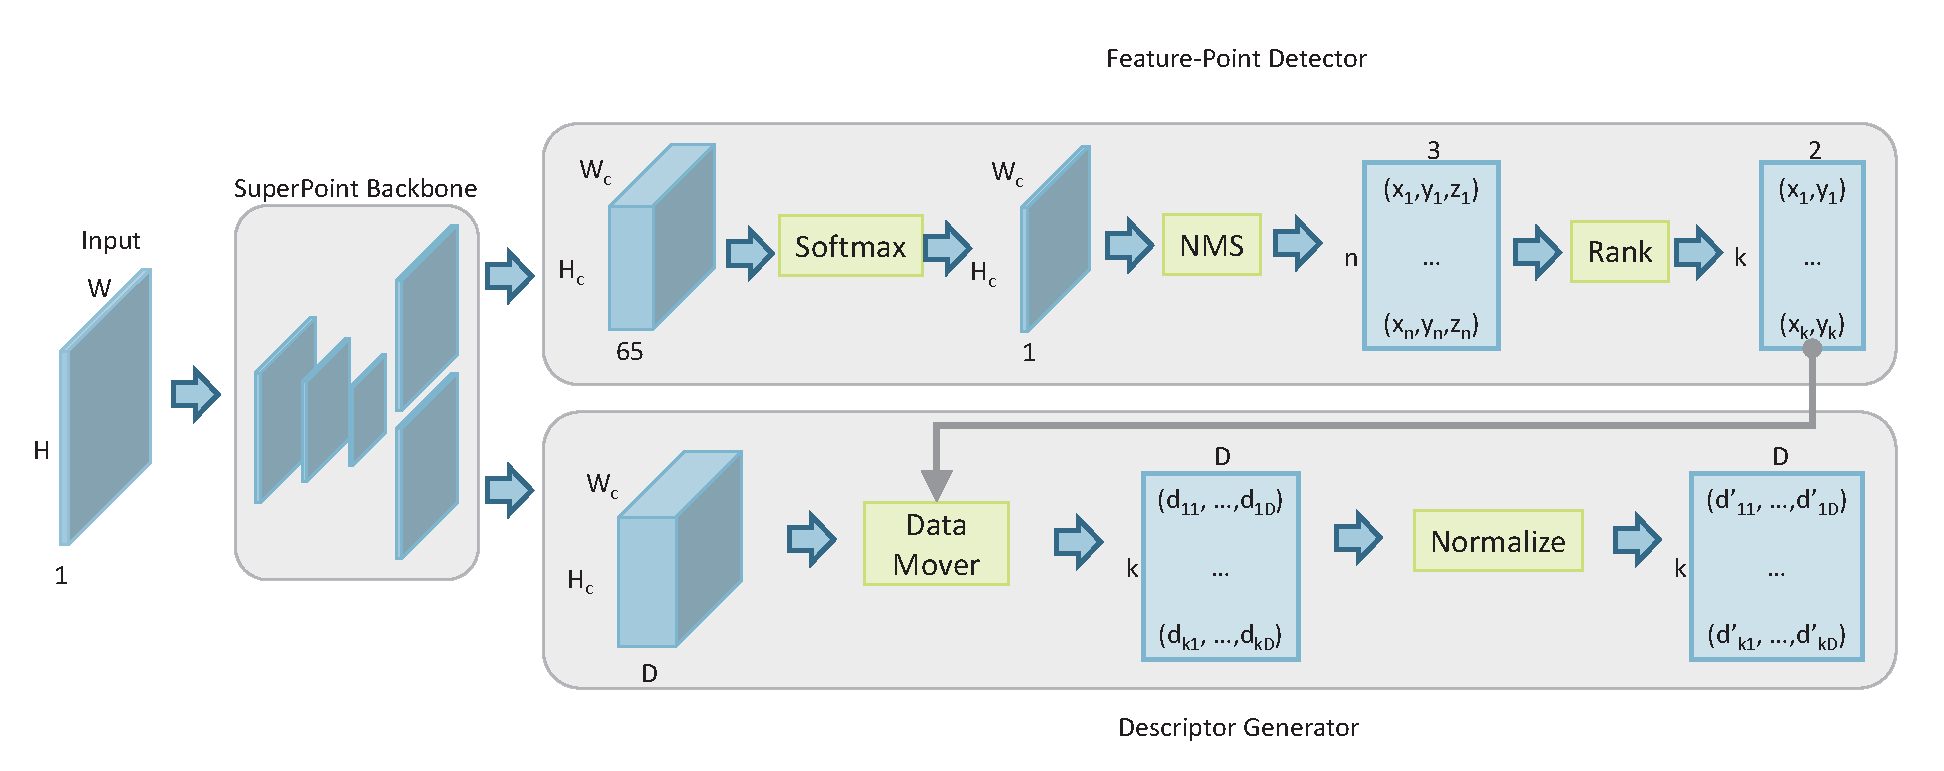
\includegraphics[width=0.95\linewidth]{fig/interexample.eps}
	\caption{ A simple example of accelerator interrupt based on Virtual Instruction. }
	\label{fig:interexample}
\end{figure*}

\subsubsection{ Virtual Filed}

Three values can be set to Virtual Filed:
\begin{itemize}
    \item[2'b00] indicates this instruction is not virtual, should always be executed.
    \item[2'b01] indicates this instruction is the SAVE instruction for backup. When an interrupt occurs, the high-priority network will start after this instruction.
    \item[2'b10] indicates this instruction is the LAOD instruction for recovery. The corresponding instructions will be executed after the high-priority network.
\end{itemize}

\subsubsection{ SaveID Filed }

SaveID links LAOD/CALC instructions to the corresponding SAVE instruction. SaveID of each not-virtual SAVE instruction differs. If the generated outputs of the LOAD/CALC are stored to DDR by a SAVE instruction, the LOAD/CALC instructions have the same SaveID as the SAVE instruction.

We consider all the LOAD/CALC instructions corresponding to one CALC\_F instruction as a \textbf{CalcBlob}. Each CalcBlob has one CALC\_F instruction, and ends up with this CALC\_F instruction. The SaveID for a CalcBlob is the same as its CALC\_F instruction.
One SAVE instruction may correspond to one CalcBlob ( \textbf{Single Blob Save}, illustrated in \Cref{fig:singlesave} ) or multiple CalcBlobs (\textbf{Multiple Blob Save}, illustrated in \Cref{fig:multisave}).

For Single Blob Save, no virtual SAVE is added. The high-priority network can be started after the nomal not-virtual SAVE. The virtual LOAD instructions for data recovery are generated after the normal SAVE, and executed after the high-priority network. The execution timeline is shown in \Cref{fig:intersinglesave}.

For Multiple Blob Save, virtual SAVE and LOAD instructions are generated after the CALC\_F of each CalcBlob. When the interrupt request occurs during the CalcBlob, the virtual SAVE instruction will be executed before the start of the high-priority network. Virtual LOAD instructions for data recovery are executed after the high-priority network. The subsequent nomal not-virtual SAVE instruction with the same SaveID as the CalcBlob will be modified to avoid duplicate output data transfer. The execution timeline is shown in \Cref{fig:intermultisave}.








\subsection{ Instruction Arrangement Unit (IAU) }

A specific hardware module called Instruction Arrangement Unit (IAU) is designed to handle the computing requirements from different tasks with different priorities. The IAU monitors the interrupt status, and generates a simple instruction sequence dynamically. The decoder, controller, processing elements in the CNN accelerator does not need to know the interrupt status, but only operate the instructions provided by IAU.

The hardware implementation of IAU is shown in \Cref{fig:IAU}, which supports four different tasks at different priorities. Task 0 has the highest priority and is uninterruptible. 

InstrAddr records the address to fetch the instructions of the corresponding task. The InputOffset and the OutputOffset are configured by the software, which indicate base address offsets of the input and output data. With the configuration of the offsets, low-latency ScratchPad memory \cite{Banakar2002Scratchpad} can be used for directly data sharing between CPU cores and accelerators. The data sharing with ScratchPad \cite{Banakar2002Scratchpad} is introduced in \Cref{sec:incame}.


SaveID, SaveAddr, and SaveLength record the backup status when an interrupt occurs. 
Subsequent not-virtual SAVE instructions will be modified according to the interrupt status recorded.
An example of the instruction modification will be given at \Cref{sec:exampleVirtual}.


\subsection{Example of Viutual Instruction}
\label{sec:exampleVirtual}


The example is based on a straightforward convolutional layer, which has only one input channel and one output channel. 
The convolution kernel size is $1 \times 1$. The shape of the input and output featuremaps is $ 2 \times 16 $ (\Cref{fig:interexample}(a) ). The two lines of output are calculated by two CALC\_F instructions ( instruction 3 and 7). The addresses used in the instruction example are listed in \Cref{fig:interexample}(b). \Cref{fig:interexample}(c) is the instruction sequence from DDR with virtual instructions. \Cref{fig:interexample}(d) is the executed instructions without interrupt. When an interrupt occurs at the first CALC\_F, \Cref{fig:interexample}(e) illustrated the backup and recovery instructions (Blue) and the modified SAVE instruction (Red).

% The hardware implementation of IAU is shouwn in \Cref{{fig:IAU}. There is a Status Pool which records the running states of each task. The InstrAddr is records the instruction address of each CNN